\documentclass[12pt,oneside,a4paper]{article}
\usepackage[spanish]{babel}
\usepackage[utf8]{inputenc}
\usepackage{graphicx}
\usepackage{amsmath}
\usepackage{amssymb}
\usepackage{color}
\usepackage{colortbl}
\usepackage{subfigure}
\usepackage{url}
\linespread{1}
\setlength{\parskip}{1\baselineskip}
\parindent 1cm
\sloppy


%Opciones que debes descomentar mientras estemos revisando el anteproyecto
%\usepackage{lineno}
%\linenumbers
%\usepackage[pagebackref=true,breaklinks=true,letterpaper=true,colorlinks,bookmarks=true]{hyperref}


%lista de palabras que Latex no parte bien
\hyphenation{pa-la-bras lis-ta}

\begin{document}

\thispagestyle{empty}

\begin{center}


Departamento de Teoría de la Señal y Comunicaciones\\
Escuela Técnica Superior de Ingeniería Informática\\
Universidad de Alcalá\\

\vspace{1cm}


\includegraphics[width=4cm]{figuras/logo-uah.eps}

\textbf{ANTEPROYECTO}

\vspace{1cm}

\begin{large}\textbf{\textit{Gestión dinámica de grupos en una plataforma de aprendizaje virtual basada en Tikiwiki}}\end{large}

\vfill

Febrero - 2011

\end{center}

\begin{flushright}
\textit{Autor - \textbf{Aldo Borrero González}} \\
\textit{Director - \textbf{Roberto Javier López Sastre}}
\end{flushright}

\newpage

\section{Introducción}

El Proyecto Fin de Carrera a desarrollar ha sido denominado \textit{Gestión dinámica de grupos en una plataforma de aprendizaje virtual basada en Tikiwiki}. El objetivo de este proyecto es permitir al usuario de Tikiwiki, a través de la herramienta conocida como \textit{Profiles}\cite{Profiles}, obtener un mayor grado de automatización cuando se trabaja con múltiples grupos que implican tareas de gestión que, de otro modo, serían costosas en esfuerzo y tiempo.

Usar esta herramienta presenta múltiples ventajas puesto que al permitir la automatización de ciertas tareas, el administrador/docente sólo necesita codificar una vez el proceso a automatizar y este puede ser aplicado una y otra vez sobre los grupos que cumplan unos ciertos requisitos. A su vez, favorece la reutilización en otras plataformas de aprendizaje virtual (basadas en Tikiwiki), puesto que dichos \textit{Profiles} pueden ser intercambiados de forma cómoda.

Gestionar grupos de una forma dinámica donde pueden coexistir múltiples permisos, reglas y excepciones, puede ser una tarea difícil, por ello se pretende explicar el funcionamiento de los \textit{Profiles} y mostrar casos de usos en los que su utilidad queda demostrada.

De cara a un docente el uso de \textit{Profiles} presenta todas las ventajas comentadas anteriormente. Por ejemplo, podría crear una asignatura (con su respectiva wiki), crear un grupo de clase asociado a esa asignatura y asignar permisos concretos al grupo. Esto se realiza de forma transparente para el docente, por lo que se abstrae de \textit{cómo} tener que llevar a cabo su tarea, y se centra en \textit{qué} quiere conseguir.

\section{Descripción del proyecto y objetivos}

En este Proyecto Fin de Carrera se pretende mostrar como funcionan los \textit{Profiles} para poder gestionar un entorno de aprendizaje virtual, en el cual un administrador de la plataforma puede llevar a cabo tareas de una manera automática y simple.

En el proyecto se tratarán de explicar las siguientes cuestiones:

\begin{itemize}
    
    \item \textbf{Código YAML\cite{YAML}}: los \textit{Profiles} basan su funcionamiento básico en el lenguaje de marcado ligero YAML, una comprensión de como este lenguaje funciona y las diferencias que presenta respecto a otros lenguajes de marcado es vital para poder entender los \textit{Profiles}.

    \item \textbf{Estudio de la arquitectura de los \textit{Profiles}}: Una vez comprendido como funciona la sintáxis de YAML, es necesario comprender como funciona un \textit{Profile} por dentro, y que impacto tiene en la plataforma de aprendizaje virtual basada en Tikiwiki.

    \item \textbf{Creación de \textit{Profiles} que automaticen tareas repetitivas para el docente}: Se crearán distintos tipos de \textit{Profiles} que hagan tareas concretas en la plataforma como la creación de una asignatura docente, creación de distintos grupos asociados a la asignatura y administración de permisos. Así mismo se darán instrucciones para que el docente cree sus propios Profiles adaptados a sus necesidades.

\end {itemize}

\begin{figure}
  \centering
  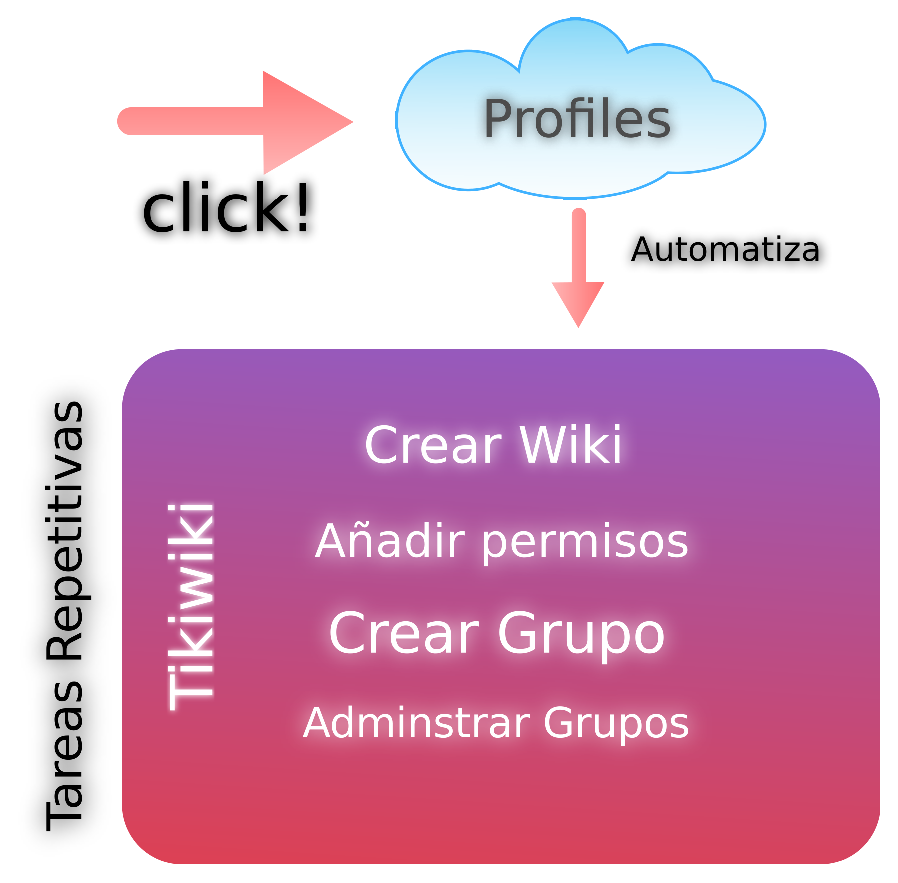
\includegraphics[width=4cm]{figuras/anteproyecto1.eps}
  \caption{Creación de una asignatura utilizando profiles en la plataforma Tikiwiki.}
  \label{fig:ejemplo}
\end{figure}


\section{Fases de desarrollo}

El proyecto \textit{Gestión dinámica de grupos en una plataforma de aprendizaje virtual basada en Tikiwiki} queda estructurado en las siguientes fases de desarrollo:

\begin{enumerate}
    
    \item Investigación de los distintos tipos de lenguaje de marcado que se pueden encontrar en la actualidad y porqué se escogió YAML.

    \item Investigación de herramientas similares a los \textit{Profiles} y que aplicabilidad tienen en un entorno de aprendizaje virtual.

    \item Creación de nuevos \textit{Profiles} que permitan construir un \textit{kit} de herramientas útiles al administrador/docente, que le permitan ahorrar tiempo en la gestión dinámica de la plataforma de aprendizaje.

    \item Implantación del modelo de gestión dinámica de grupos en la plataforma de aprendizaje virtual ALMA\cite{ALMA}.

    \item Fase de pruebas y depuración.

    \item Edición del documento final utilizando \LaTeX.
\end{enumerate}

%Bibliografía
\begin{thebibliography}{9}
    \bibitem{Profiles} Comunidad de Tikiwiki. Profiles en la comunidad de Tikiwiki: www.profiles.tikiwiki.org, 2009.

    \bibitem{YAML} YAML Consortium. Página oficial de YAML: www.yaml.org, 2010.
    
    \bibitem{ALMA} Proyecto ALMA, www2.uah.es/alma/wikis.html, 2011

\end{thebibliography}

\end{document}
